Without certificate authorities and X.509, users would be at risk from having  their TCP connections (SMTP,HTTP, etc) hijacked or compromised. X.509 and certificate authorites are characteristics of public key infrastructure (PKI) schema.\\
\subsection{Overview of PKI Model}
PKI is an infrastructure that provide internet users with the means to securely and privately exchange information through the use of a public and a private key pair obtained and shared through a trusted authority. It also provides digital certificates that matches an individual or organization, a reporsitory that strores and when necessary can revoke the certficates.The component of a public key infrastructure are:\\
End Entity : \indent Users, organizations, or systems who intends to use the private and public technology to securely exchange information.\\
Certificate Authority(CA) : \indent  The oraganization that issues digital certificates binding subject's identity with subjects's public key.\\
Registration Authority(RA) : \indent An optional system to which CA delegate some functions like verifying the subject's identity.\\
Certificate Revocation List(CRL) Issuer: \indent An optional system to which CA delegate the function to publish the Certificate revocation list containing certificates revoked by the CA.\\
Validation Authority(VA) : \indent An optional system to which CA delegate some functions like verifying the digital certificate subject.\\

\begin{figure}[h]
\centering
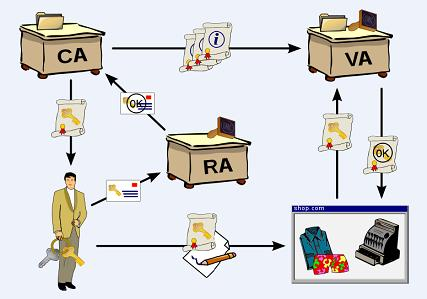
\includegraphics[width=0.7\linewidth]{./figures/PKI_Introduction}
\caption[PKI Workflow]{}
\label{fig:PKI_Introduction}
\end{figure}

\subsection{X.509 Certificate Format}
\subsection{Certificate Validation Process}
\subsection{Subordinate Certificate Authority(SubCA) or Intermidiary CA}

